% !TEX encoding = UTF-8 Unicode
\documentclass[12pt]{article}
\usepackage{flafter}
\usepackage{color}
\usepackage{url}
\usepackage{float}
\usepackage[T2A]{fontenc} % enable Cyrillic fonts
\usepackage[utf8]{inputenc} % make weird characters work
\usepackage{graphicx}
\usepackage{multirow}
\usepackage[english,serbian]{babel}
%\usepackage[english,serbianc]{babel} %ukljuciti babel sa ovim opcijama, umesto gornjim, ukoliko se koristi cirilica
\usepackage[margin=1in]{geometry}
\usepackage[unicode]{hyperref}
\hypersetup{colorlinks,citecolor=green,filecolor=green,linkcolor=blue,urlcolor=blue}

\usepackage{listings}
\usepackage{multirow}
\newcommand\todos[1]{\textcolor{red}{#1}}

%\newtheorem{primer}{Пример}[section] %ćirilični primer
\newtheorem{primer}{Primer}[section]

\definecolor{mygreen}{rgb}{0,0.6,0}
\definecolor{mygray}{rgb}{0.5,0.5,0.5}
\definecolor{mymauve}{rgb}{0.58,0,0.82}



\lstset{ 
	backgroundcolor=\color{white},   % choose the background color; you must add \usepackage{color} or \usepackage{xcolor}; should come as last argument
	basicstyle=\footnotesize,        % the size of the fonts that are used for the code
	breakatwhitespace=false,         % sets if automatic breaks should only happen at whitespace
	breaklines=true,                 % sets automatic line breaking
	captionpos=b,                    % sets the caption-position to bottom
	commentstyle=\color{mygreen},    % comment style
	deletekeywords={...},            % if you want to delete keywords from the given language
	escapeinside={\%*}{*)},          % if you want to add LaTeX within your code
	extendedchars=true,              % lets you use non-ASCII characters; for 8-bits encodings only, does not work with UTF-8
	firstnumber=1000,                % start line enumeration with line 1000
	frame=single,	                   % adds a frame around the code
	keepspaces=true,                 % keeps spaces in text, useful for keeping indentation of code (possibly needs columns=flexible)
	keywordstyle=\color{blue},       % keyword style
	language=Python,                 % the language of the code
	morekeywords={*,...},            % if you want to add more keywords to the set
	numbers=left,                    % where to put the line-numbers; possible values are (none, left, right)
	numbersep=5pt,                   % how far the line-numbers are from the code
	numberstyle=\tiny\color{mygray}, % the style that is used for the line-numbers
	rulecolor=\color{black},         % if not set, the frame-color may be changed on line-breaks within not-black text (e.g. comments (green here))
	showspaces=false,                % show spaces everywhere adding particular underscores; it overrides 'showstringspaces'
	showstringspaces=false,          % underline spaces within strings only
	showtabs=false,                  % show tabs within strings adding particular underscores
	stepnumber=2,                    % the step between two line-numbers. If it's 1, each line will be numbered
	stringstyle=\color{mymauve},     % string literal style
	tabsize=2,	                   % sets default tabsize to 2 spaces
	title=\lstname                   % show the filename of files included with \lstinputlisting; also try caption instead of title
}

\begin{document}
	
	\title{Rešavanje problema optimalnog planiranja kretanja u grafu primenom genetskog algoritma \\ \large{Seminarski rad u okviru kursa Računarska inteligencija \\Matematički fakultet}}

	\author{Petrović Ana, Spasojević Đorđe\\pana.petrovic@gmail.com, djordje.spasojevic1996@gmail.com}
	
	%\date{9.~april 2015.}
	
	\maketitle
	\thispagestyle{empty}
	\vspace*{2\baselineskip}
	\abstract{
	U ovom radu predstavljen je genetski algoritam prilagođen problemu optimalnog planiranja kretanja u povezanom, neusmerenom, acikličnom grafu. Cilj je pronaći rešenje koje u najmanjem broju poteza dovodi robota od početnog čvora do cilja, uz izbegavanje prepreka koje se takođe mogu pomerati. Najpre su prikazani pojedinačni koraci genetskog algoritma, a zatim i testiranje kvaliteta rešenja u zavisnosti od promene različitih parametara. Rezultati pokazuju da genetski algoritam relativno uspešno rešava postojeći problem, kao i da u zavisnosti od tipa grafa, menjanje različitih parametara može uticati na kvalitet rešenja. 
	} 
\newpage
	\tableofcontents
	
	\newpage
	
	\section{Uvod}
	\label{sec:uvod}  
	\par Planiranje kretanja (eng. \textit{Motion Planning}) predstavlja jedan od opštih problema u oblasti robotike, čija postavka podrazumeva postojanje robota kojeg treba dovesti od početne tačke do cilja, uz izbegavanje postojećih prepreka \cite{def}. U literaturi je prethodno ponuđeno više rešenja za ovaj problem primenom genetskog algoritma 
	\cite{gen2, gen1, gen3}. Iako nijedan od ovih pristupa nije sasvim primenjiv na konceptualizaciju našeg problema, svakako su nam ovi radovi pomogli da bolje razumemo i genetski optimizujemo sam problem. 
	\par U ovom radu, dati problem je specifikovan tako da je  potrebno naći sekvencu validnih poteza u povezanom, neusmerenom grafu. Radi pojednostavljivanja pronalaženja rešenja, odabrano je da se u primerima koriste samo aciklični grafovi. Graf se sastoji od unapred određenog broja čvorova, od koji svaki može u jednom trenutku da sadrži ili robota, ili prepreku, ili može biti slobodan. Jedan potez podrazumeva premeštanje robota ili prepreke u susedni slobodni čvor. Cilj je pronaći rešenje koje u najmanjem broju poteza dovodi robota od početnog čvora, označenog kao S, do ciljnog čvora, označenog kao T \cite{glavni}. 
	Na slici \ref{fig:slika1} je prikazan jednostavan primer postavke jednog ovakvog problema. U svim grafovima koje ćemo koristiti kao primere, čvor je crvene boje ako je na njemu trenutno prepreka, robot se nalazi na plavom čvoru, a ciljni čvor je obojen zelenom bojom dok je slobodan.
	\vspace*{1\baselineskip}
	\begin{figure}[h!]
		\begin{center}
			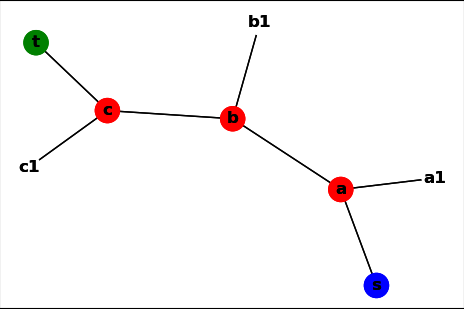
\includegraphics[scale=1]{graf.png}
		\end{center}
		\caption{Primer postavke problema planiranja kretanja u grafu}
		\label{fig:slika1}
	\end{figure}
	
	\newpage
	\section{Opis algoritma}
	\label{sec:prvoPoglavlje}
	\par U radu je dat predlog rešenja korišćenjem genetskog algoritma. Prvi korak, koji je ujedno i jedan od najvažnijih u genetskom algoritmu jeste određivanje načina na koji 
	će jedinka (hromozom) biti predstavljena. Od reprezentacije hromozoma značajno zavisi ponašanje algoritma. Nakon toga, najčešće nasumično, generiše se početna populacija koja se sastoji od određenog broja jedinki. U narednom koraku, računa se kvalitet svake jedinke, tj. funkcija prilagođenosti, a na osnovu nje se vrši selekcija najprilagođenijih jedinki iz populacije. Potom se nad selektovanim jedinkama primene genetski operatori ukrštanja i mutacije, kojima se formiraju nove generacije, sve dok se ne dostigne neki kriterijum zaustavljanja i pronađe najbolje rešenje u datom trenutku.
	
	\subsection{Reprezentacija jedinke}
	\label{subsec:podnaslov1}
	Pri generisanju početne populacije, razmatrani su različiti načini predstavljanja rešenja. U većini prethodnih radova autori predlažu hromozom u obliku koordinata pozicija robota, ili putanje od početnog do krajnjeg čvora. 
	Takva reprezentacija se nije dobro pokazala u našem slučaju, s obzirom na to da se prepreke mogu kretati na isti način kao i robot, kao i da postoji samo jedan put od čvora S do čvora T, jer je u pitanju aciklički graf.
	\par Zbog toga, početnu populaciju u našem algoritmu čine jedinke koje predstavljaju neku nasumičnu putanju, odnosno niz različitih validnih poteza, koji počinju od početnog stanja grafa. Preciznije, jedinka se sastoji od pokreta robota ili prepreka, koji su predstavljeni preko izvornog čvora, ciljnog čvora, težine puta između ta dva čvora i liste koja predstavlja celu putanju. Na primer, potez od čvora A do čvora B bi bio dat u obliku četvorke ('A', 'B', 1, ['A', 'B']). U slučaju pomeranja prepreka, dozvoljeni su potezi i veće težine od 1, jer je prethodno dokazano da kada je potrebno da se prepreka premesti u neki slobodan čvor (koji joj nije susedan), broj poteza je isti kao i dužina puta između ta dva čvora. Ono što je bitno u tom slučaju je da je na kraju tih poteza stanje grafa takvo da je polazni čvor slobodan, a ciljni zauzet preprekom \cite{glavni}.
	\par Svaka od putanja u populaciji kreće od početnog stanja i zatim se za svaki naredni potez robota ili prepreke najpre razmatra da li je potez validan iz trenutnog stanja grafa, tj. trenutne pozicije prepreka i robota. Generiše se lista svih mogućih poteza iz trenutnog stanja i nasumično bira jedan iz liste. Zatim se izvrši taj potez i dobija se novo stanje grafa. Ako je novo stanje takvo da se robot nalazi u ciljnom čvoru, ne traže se naredni mogući potezi, jer je pronađeno rešenje. Ako je to stanje već ranije bilo razmatrano za tu jedinku, takav potez ne dodajemo u nju, jer ne želimo da se stanja ponavljaju. Može se desiti da se ovakvim nasumičnim dodavanjem istroše sva moguća stanja grafa i da više ne može da se doda nijedan potez.
	Iz tog razloga, dužina hromozoma neće biti fiksna, jer postoje slučajevi kada više neće biti validnih poteza iz nekog stanja. Maksimalna dužina jednog hromozoma ChromosomeLength određena je tako da bude proizvod dužine putanje od početnog čvora do ciljnog čvora, u oznaci P, i broja prepreka O koje se nalaze na toj putanji. \newline
	
	$ ChromosomeLength =  P * O $  \newline
	
	
	\subsection{Funkcija prilagođenosti}

	\label{sec:drugoPoglavlje}
	Svakoj jedinki dodeljuje se skor, čija visina ukazuje na prilagođenost jedinke. Skor se računa na osnovu poteza koji čine tu jedinku, i stanja grafa nakon tih izvršenih poteza, odnosno mesta na kojima se nalaze prepreke i robot nakon što su potezi izvršeni. Funkcija kao parametar prima i putanju od početnog do ciljnog čvora \textit{path}. Najpre se izračuna ukupna dužina putanje koja čini jedinku \textit{weight}, i skor se na početku postavi na \textit{-weight}.
	Zatim se proverava da li je trenutno stanje robota jednako ciljnom čvoru T. Ukoliko se robot nalazi na cilju, skoru se dodaje neki određeni visok broj SOLVED\_AWARD. Zatim se proverava da li je robot lociran na glavnoj putanji između početnog i ciljnog čvora, za šta se takođe dodaje određena vrednost na postojeći skor. Uz to, ukoliko se na tom putu nalazi neka prepreka, za svaku od njih se skor umanjuje za određenu vrednost. Ukoliko se nijedna prepreka ne nalazi na glavnom putu, a uz to je i ciljni čvor T slobodan, skor se povećava za određenu vrednost. Pored toga, proverava se da li se robot kreće ka cilju kada mu je oslobođena putanja i za svaki potez ka cilju povećava se skor.
	\vspace*{1\baselineskip}
	\lstinputlisting[language=Python, caption = Fitnes funkcija]{fitness.py}
	
	\subsection{Selekcija}	
	Pri selekciji, vrši se izbor jedinki iz trenutne populacije za reprodukciju. U našem radu korišćena je turnirska selekcija. Turnirska selekcija podrazumeva da jedinke učestvuju u turnirima, a u svakom od njih, najbolje prilagođena jedinka se proglašava pobednikom. Veličina turnira zadata je parametrom tournament\_size. U listu selektovanih jedinki se dodaju pobednici turnira sve dok veličina liste ne dostigne parametar reproduction\_size. 
	\vspace*{1\baselineskip}
	\lstinputlisting[language=Python, caption = Turnirska selekcija]{selection.py}
	
	
	\subsection{Kreiranje nove generacije}	
	\label{sec:trecePoglavlje}
	
	Pri kreiranju nove generacije, korišćena je strategija elitizma. Njome se obezbeđuje da se kvalitet rešenja ne smanjuje iz generacije u generaciju, tako što se uvek u narednu generaciju direktno prenosi određeni broj najbolje prilagođenih jedinki. U našem algoritmu, broj elitnih jedinki je velik (na primer, polovina veličine populacije) jer se pri generisanju populacije stvaraju veoma nasumične jedinke, s obzirom da se pri svakom potezu u potpunosti menja stanje grafa, odnosno menja se svaki mogući legitimni potez. Na ostale jedinke u populaciji koje ne prelaze direktno u narednu generaciju, primenjuje se operator ukrštanja, tako što se od prethodno selektovanih jedinki odabiraju dve nasumično, i one postaju roditelji. U ukrštanje će ulaziti samo jedinke koje su veće od neke minimalne dužine, da bi mogle da se iseku na nekoj nasumičnoj poziciji u procesu ukrštanja. Mutaciju primenjujemo i na jednu nasumičnu elitnu jedinku, i na dete koje nastane procesom ukrštanja.
	\vspace*{1\baselineskip}
	\lstinputlisting[language=Python, caption = Generisanje nove generacije]{newgen.py}
	
	\subsubsection{Ukrštanje}
	\label{subsec:podnaslov2}
	
	Kako postoji velik broj elitnih jedinki, ukrštanje se vrši nad manjim brojem jedinki iz populacije. U našem algoritmu korišćeno je jednopoziciono ukrštanje, tako što je roditelj čija je putanja kraća presečen na nasumično odabranoj poziciji \textit{i}. Deo poteza do \textit{i} iz prvog roditelja mora da se izvrši da se dobije novo stanje grafa. Nakon toga, polazi se od \textit{i-te} pozicije u drugom roditelju i za svaki pojedinačan potez proverava da li je moguć iz prethodno dobijenog stanja. Ovde nastaje problem, jer svaki put mora da se izvrši i doda novi potez na trenutno stanje, čime se dobija potpuno novo stanje. Dete će se dopunjavati dokle god je to moguće, ali u velikom broju slučajeva potezi iz drugog roditelja neće biti mogući u datom stanju. Tako dete koje nastaje često može biti lošijeg kvaliteta od roditelja. Upravo iz tog razloga i koristimo elitizam sa tako velikim procentom. Za svaki novi potez iz drugog roditelja potrebno je proveriti da li je moguć u odnosu na \textit{sve} prethodne, i samo ako jeste, može da se doda jedan potez, a već za sledeći možda opet neće biti moguće. Parametri funkcije ukrštanja su
	prvi roditelj, drugi roditelj, stanje prepreka, stanje robota, graf, ciljni čvor, veličina populacije i putanja od prvog do poslednjeg čvora.

	\lstinputlisting[language=Python, caption = Ukrštanje]{cross.py}
	
	
	\subsubsection{Mutacija}
	\label{subsec:podnaslov3}
	
	Mutacija podrazumeva malu promenu genoma koja se dešava sa jako malom verovatnoćom, a koja omogućava različitost u narednoj generaciji i izbegavanje zaglavljivanja u lokalni optimum. U našem slučaju, mutacija će biti jednostavno dodavanje samo jednog poteza iz liste svih mogućih u trenutnom stanju, nakon izvršenih poteza do tog trenutka. Putanje su se nekad skraćivale u ukrštanju, pa će ih dodavanje jednog poteza povećavati s vremena na vreme. Funkcija za parametre ima jedinku \textit{chromosome}, stanje prepreka \textit{o}, stanje robota \textit{r}, graf \textit{graph}, veličinu populacije \textit{population\_size}, putanju \textit{path}, i ciljni čvor \textit{t}. Na početku se izvrše svi potezi iz jedinke da bi se dobilo novo stanje. Proveri se da li je novo stanje robota jednako t, i ako jeste izlazi se iz funkcije jer ne želimo da mutiramo jedinku koja je pronašla rešenje. Ako nije, uzima se prvi potez iz liste svih mogućih poteza iz datog stanja koji predstavlja kretanje robota, jer najviše želimo da se robot kreće, a ako ne postoji takav potez onda se uzima bilo koji drugi koji nije vraćanje u prethodan čvor (funkcija \textit{different\_moves}). Nakon dodavanja poteza, potrebno je da se ponovo izvrše svi potezi sa novim dodatim, i nakon toga odredi skor novonastale jedinke. 
	\vspace*{1\baselineskip}
	\lstinputlisting[language=Python, caption = Mutacija]{mutation.py}
	


	\subsection{Prikaz algoritma}
	\label{sec:cetvrtoPoglavlje}
	U nastavku je dat kod funkcije koja radi optimizaciju, odnosno objedinjuje sve prethodno opisane korake i izvršava ih sve dok nije postignut kriterijum zaustavljanja, koji je odabran da bude neki maksimalan broj iteracija. Parametri funkcije su stanje prepreka \textit{o}, stanje robota \textit{r}, graf \textit{graph}, ciljni čvor \textit{t}, i putanja od početnog do ciljnog čvora \textit{path}.
	\vspace*{2\baselineskip}
	\lstinputlisting[language=Python, caption = Genetski algoritam]{solver.py}

	\section{Rezultati}
	U ovom poglavlju biće prikazani rezultati izvršavanja algoritma na različitim primerima. Koristićemo 3 različite postavke problema, i menjati neke od parametara da bismo zaključili kako koji utiče na kvalitet rešenja. Kao ocenu kvaliteta rešenja izdvajamo broj generacije u kojoj je pronađeno to rešenje, broj poteza za koje se izvršava i vreme izvršavanja u sekundama. Primere ćemo nazvati G1, G2 i G3. Primeri problema dati su na slikama \ref{fig:slika2}, \ref{fig:slika3}, \ref{fig:slika4}.  
	
		\begin{figure}[h]
		\begin{center}
			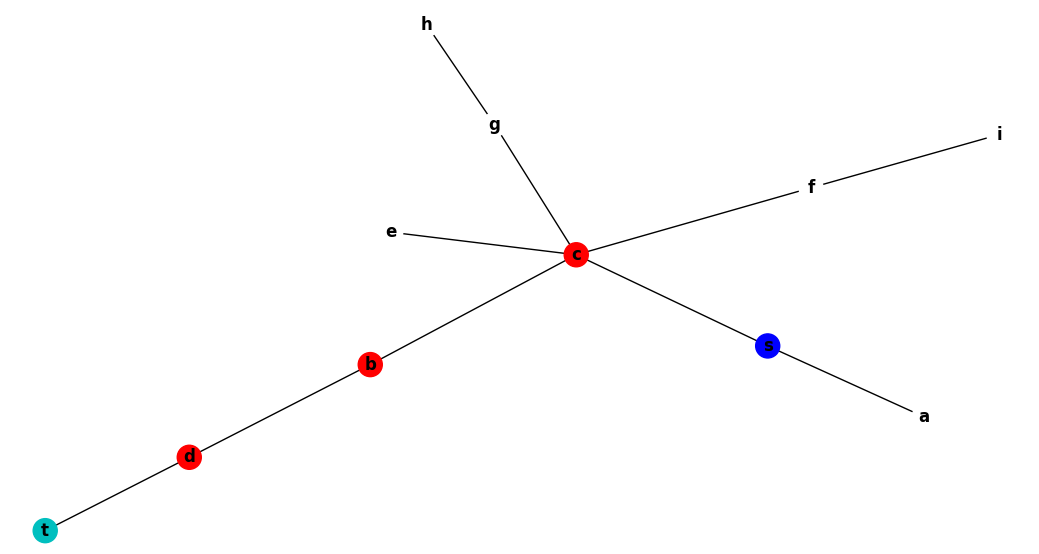
\includegraphics[scale=0.45]{g1.png}
		\end{center}
		\caption{Primer G1}
		\label{fig:slika2}
	\end{figure}
	


	Za sva tri primera podrazumevana je veličina populacije 200, broj elitnih jedinki je 20, maksimalan broj iteracija je 500, veličina za reprodukciju je 30, veličina turnira 5, verovatnoća mutacije 10\%.
	\par Kao što se vidi u Tabeli 1, bez obzira na verovatnoću mutacije, do rešenja se uvek stiže u istom broju poteza. Međutim, kada je verovatnoća mutacije 10\%, do rešenja se stiže najbrže, odnosno u 12. generaciji, te ovo može sugerisati da je ova visina kriterijuma verovatnoće mutacije najoptimalnija za pronalaženje rešenja. 
	
	\begin {table}[H]
	\begin{center}
	\caption {Rezultati za G1 sa promenom parametra mutacije} \label{tab:title} 
	\begin{tabular}{|| c|c c c||} 	
		\hline
		& M = 5\% & M = 10\% & M = 20\% \\ 
		\hline\hline
		Generacija & 16 & 12 & 22  \\ 
		\hline
		Broj poteza & 15 & 15 & 15 \\
		\hline
		Vreme izvršavanja & 25.871 & 28.319 & 20.389 \\
		\hline
	\end{tabular}
	\end{center}
	\end{table}
	\par
	\par S obzirom da se radi o jednostavnom grafu, rešenje će se pronaći u nekoj od ranijih generacija, te parametar broja iteracija može biti postavljen na 50. Međutim, ovo ne garantuje najoptimalnije rešenje, s obzirom da kasnije generacije mogu unaprediti kvalitet rešenja, što se vidi u slučaju kada je parametar postavljen na 200. 
		\begin {table}[H]
	\begin{center}
		\caption {Rezultati za G1 sa promenom broja iteracija} \label{tab:title} 
		\begin{tabular}{|| c|c c c||} 	
			\hline
			& maxIt = 50 & maxIt = 200 & maxIt = 500 \\ 
			\hline\hline
			Generacija & 6 & 14 & 22  \\ 
			\hline
			Broj poteza & 17 & 15 & 15 \\
			\hline
			Vreme izvršavanja & 3.458 & 8.251 & 20.389 \\
			\hline
		\end{tabular}
	\end{center}
\end{table}
	\par
	\par Kao što Tabela 3 pokazuje, kada je populacija najveća, do rešenja se stiže veoma rano. Za razliku od toga, kada je populacija manja, do rešenja se dolazi kasnije, a uz to je ono za najmanju populaciju i najlošijeg kvaliteta. S obzirom na jednostavnost problema, može se izabrati i manja populacija, kako se ne bi gubilo vreme na kreiranje incijalne populacije.
	\begin {table}[H]
	\begin{center}
		\caption {Rezultati za G1 sa promenom veličine populacije} \label{tab:title} 
		\begin{tabular}{|| c|c c c||} 	
			\hline
			& popSize = 50 & popSize = 200 & popSize = 1000 \\ 
			\hline\hline
			Generacija & 12 & 78 & 2 \\ 
			\hline
			Broj poteza & 25 & 15 & 17 \\
			\hline
			Vreme izvršavanja & 2.39 & 9.36 & 66.1 \\
			\hline
		\end{tabular}
	\end{center}
\end{table}
	

\begin{figure}[h!]
	\begin{center}
		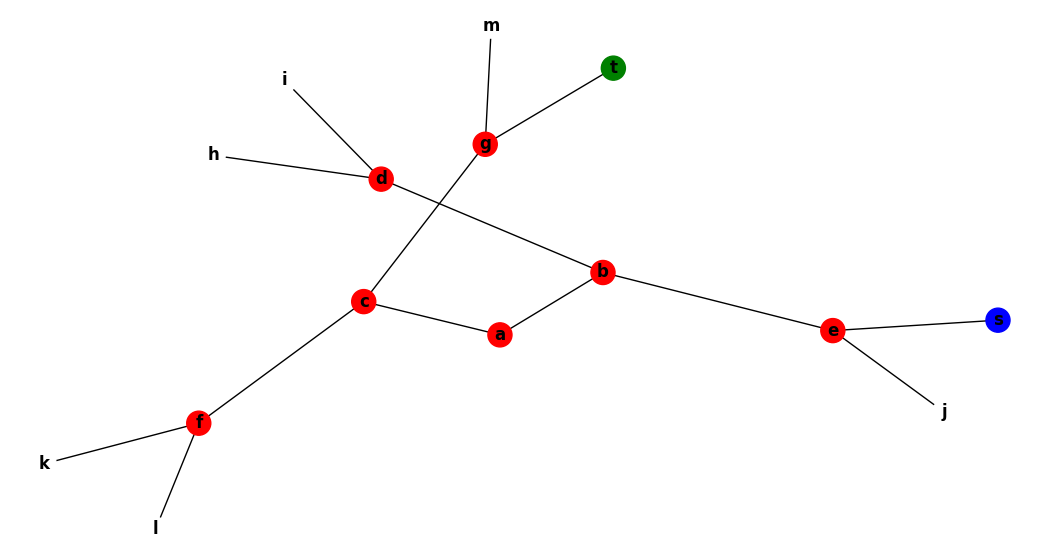
\includegraphics[scale=0.45]{g2.png}
	\end{center}
	\caption{Primer G2}
	\label{fig:slika3}
\end{figure}

 \par U Tabeli 4 nalaze se rezultati variranja verovatnoće mutacije za primer G2. Kao što tabela pokazuje, kada je verovatnoća mutacije najniža, dobija se i najbolje rešenje. U ovom slučaju, ovaj parametar predstavlja najbolje rešenje jer je priroda grafa takva - kako postoji veliki broj prepreka, ne želimo da se one prečesto nasumično pomeraju, što je ono što mutacija zapravo radi. 

	\begin {table}[H]
	\begin{center}
		\caption {Rezultati za G2 sa promenom parametra mutacije} \label{tab:title} 
		\begin{tabular}{|| c|c c c||} 	
			\hline
			& M = 5\% & M = 10\% & M = 20\% \\ 
			\hline\hline
			Generacija & 9 & 5 & 20  \\ 
			\hline
			Broj poteza & 15 & 21 & 18 \\
			\hline
			Vreme izvršavanja & 22.833 & 28.141 & 21.351 \\
			\hline
		\end{tabular}
	\end{center}
\end{table}

	\par U Tabeli 5 se nalaze rezultati promene broja iteracija za graf G2. Ova tabela nije mnogo informativna, s obzirom da će se rešenja pronaći relativno rano, te nam nije neophodan veliki broj iteracija. 

	\begin {table}[H]
\begin{center}
	\caption {Rezultati za G2 sa promenom broja iteracija} \label{tab:title} 
	\begin{tabular}{|| c|c c c||} 	
		\hline
		& maxIt = 50 & maxIt = 100 & maxIt = 500 \\ 
		\hline\hline
		Generacija & 19 & 14 & 7  \\ 
		\hline
		Broj poteza & 16 & 21 & 16\\
		\hline
		Vreme izvršavanja & 9.85 & 17.50 & 45.87 \\
		\hline
	\end{tabular}
\end{center}
\end{table}

	\par Tabela 6 pokazuje da kada je populacija manja, do rešenja se stiže u kasnijim generacijama, što sugeriše da bi u ovom slučaju bilo korisno uzeti veću veličinu populacije, slično kao i u prvom primeru. 

\begin {table}[H]
\begin{center}
\caption {Rezultati za G2 sa promenom veličine populacije} \label{tab:title} 
\begin{tabular}{|| c|c c c||} 	
	\hline
	& popSize = 200 & popSize = 500 & popSize = 1000 \\ 
	\hline\hline
	Generacija & 20 & 9 & 9 \\ 
	\hline
	Broj poteza & 18 & 18 & 17 \\
	\hline
	Vreme izvršavanja & 63.7 & 8.25 & 129.84 \\
	\hline
\end{tabular}
\end{center}
\end{table}

\begin{figure}[H]
	\begin{center}
		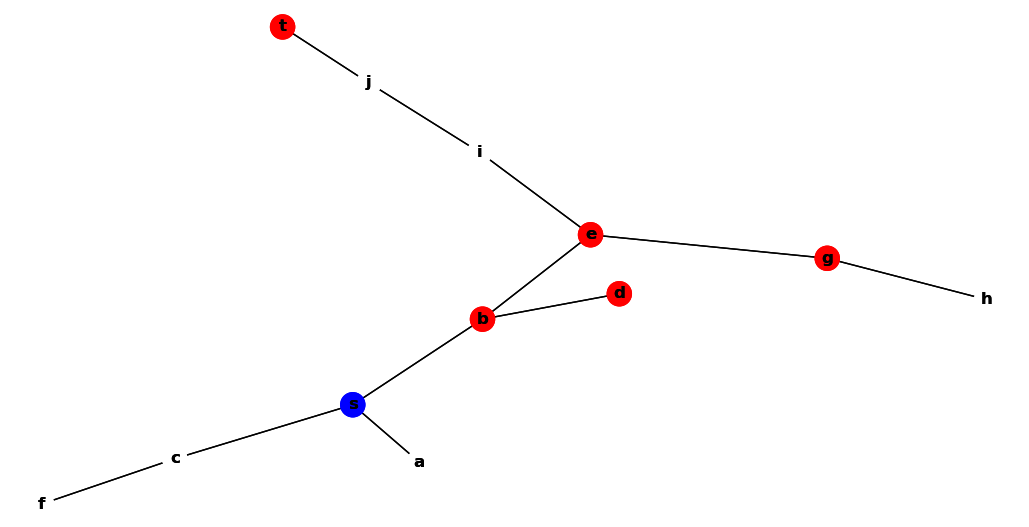
\includegraphics[scale=0.42]{g3.png}
	\end{center}
	\caption{Primer G3}
	\label{fig:slika4}
\end{figure}

 \par Treći graf je najkompleksniji za rešavanje, odnosno robot može često zapasti u zaglavljeno stanje. Zbog toga je bolje parametar podesiti na veću verovatnoću mutacije, jer se njome obezbeđuje nasumično pomeranje prepreke, što može dovesti do oslobođenja puta robotu, o čemu svedoče rezultati u Tabeli 7. 

	\begin {table}[H]
\begin{center}
	\caption {Rezultati za G3 sa različitim parametrom mutacije} \label{tab:title} 
	\begin{tabular}{|| c|c c c||} 	
		\hline
		& M = 5\% & M = 10\% & M = 20\% \\ 
		\hline\hline
		Generacija & 190 & 89 & 17  \\ 
		\hline
		Broj poteza & 41 & 26 & 40 \\
		\hline
		Vreme izvršavanja & 15.704 & 24.09 & 23.999 \\
		\hline
	\end{tabular}
\end{center}
\end{table}

	\par Rezultati u Tabeli 8 svedoče o tome da ovakva vrsta problema zahteva veći broj iteracija, s obzirom da se problem ne rešava kada je broj iteracija 50. Kada je broj iteracija postavljen na 200, vidimo da se pronalazi rešenje, koje je čak i bolje nego ono koje dobijamo kada je broj iteracija 500. 

	\begin {table}[H]
\begin{center}
	\caption {Rezultati za G3 sa promenom broja iteracija} \label{tab:title} 
	\begin{tabular}{|| c|c c c||} 	
		\hline
		& maxIt = 50 & maxIt = 200 & maxIt = 500 \\ 
		\hline\hline
		Generacija &  nije rešen & 89 & 73  \\ 
		\hline
		Broj poteza &  nije rešen& 26 & 40\\
		\hline
		Vreme izvršavanja & 8.10 & 24.09 & 49.87 \\
		\hline
	\end{tabular}
\end{center}
\end{table}

	\par Tabela 9 pokazuje da je populacija od 50 mala, ali da se sa većim populacijama, od 200 i 1000 jedinki brzo dolazi do rešenja. 

\begin {table}[H]
\begin{center}
\caption {Rezultati za G3 sa promenom veličine populacije} \label{tab:title} 
\begin{tabular}{|| c|c c c||} 	
	\hline
	& popSize = 50 & popSize = 200 & popSize = 1000 \\ 
	\hline\hline
	Generacija & 33 & 4 & 6 \\ 
	\hline
	Broj poteza & 40 & 38 & 20 \\
	\hline
	Vreme izvršavanja & 6.18 & 32.41 & 93.064 \\
	\hline
\end{tabular}
\end{center}
\end{table}
		
		
\vspace*{2\baselineskip}
Uporedićemo vreme izvršavanja našeg algoritma u odnosu na algoritam grube sile, za sva tri primera. Kao što je rečeno, najbolje moguće rešenje obično bude pronađeno već u ranim iteracijama, tako da nije potrebno iterirati do poslednje kao što smo u prethodnim testovima. Dakle, pri poređenju algoritma sa algoritmom grube sile, algoritam se završava čim se pronađe dovoljno dobro rešenje.
	\par Kao što se vidi u Tabeli 10, što graf ima više čvorova, to će algoritam grube sile duže raditi, te u ovom i njemu sličnim primerima, genetski algoritam predstavlja dobru optimizaciju - ne pronalazi najbolje rešenje, ali pronalazi dovoljno dobro rešenje, u značajno kraćem vremenskom intervalu. U druga dva primera, koji imaju manji broj čvorova, genetski algoritam ne pruža značajno poboljšanje u odnosu na algoritam grube sile, što je i očekivano. 

	\begin {table}[H]
\begin{center}
	\caption {Vreme izvršavanja u sekundama u odnosu na algoritam grube sile} \label{tab:title} 
	\begin{tabular}{|| c|c c c||} 	
		\hline
		& Gruba sila & Genetski algoritam & \\ 
		\hline\hline
		Graf G1 &  0.146 & 0.177 & \\ 
		\hline
		Graf G2 & 29.084 & 5.068 & \\
		\hline
		Graf G3 & 0.53 & 1.73 & \\
		\hline
	\end{tabular}
\end{center}
\end{table}


\vspace*{3\baselineskip}
Primer G3 se pokazao kao najteži za rešavanje. U nastavku su dati grafički prikazi učestalosti dobrih i loših rešenja primera G3 u 100 puštanja programa. Parametri za ovih 100 rešenja su birani kao optimalni za ovaj primer i dati su u Tabeli 11. Kao i ranije, program se prekida u trenutku kada se naiđe na neko dovoljno dobro rešenje. Na slici \ref{fig:slika5} prikazan je histogram učestalosti generacija u kojima je pronađeno to rešenje. Može se videti da se preko 40 puta desilo da je rešenje pronađeno između 20. i 30. generacije, i preko 10 puta u prvih 20 generacija. Manje od 10 puta rešenje je pronađeno u poslednjih 10 generacija. Histogram sa slike  \ref{fig:slika6} pokazuje vremena izvršavanja svakog od izvršavanja. Može se zaključiti da je prosek pronalaska dovoljno dobrog rešenja za G3 između 4 i 6 sekundi. Na samom kraju, slika \ref{fig:slika7} prikazuje učestalosti brojeva poteza u rešenjima za svako od izvršavanja, tj. optimalnost dobijenih rešenja. U više od 50\% slučajeva, broj poteza je između 20 i 30, što se može smatrati dobrim rešenjem, s obzirom na to da je optimalno rešenje za G3 18 poteza. Na histogramu se vidi da je to rešenje čak i pronađeno u jednom od 100 izvršavanja. Algoritam je samo 3 puta vratio loše rešenje od preko 100 poteza.

	\begin {table}[H]
\begin{center}
	\caption {Parametri za 100 puštanja programa} \label{tab:title} 
	\begin{tabular}{|| c|c ||} 	
		\hline\hline
		Veličina populacije &  200   \\ 
		\hline
		Broj elitnih jedinki & 50   \\
		\hline
		Maksimalan broj iteracija & 200   \\
		\hline
		Broj jedinki za reprodukciju  & 30   \\
		\hline
		Veličina turnira & 10   \\
		\hline
		Verovatnoća mutacije & 20\%  \\ 
		\hline
	\end{tabular}
\end{center}
\end{table}


	\begin{figure}[H]
	\begin{center}
		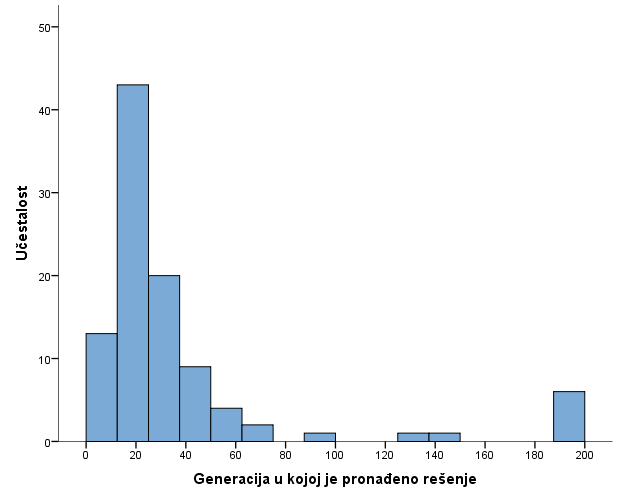
\includegraphics[scale=0.4]{generacije1.png}
	\end{center}
	\caption{{\small Histogram učestalosti generacija za 100 puštanja programa za G3}}
	\label{fig:slika5}
\end{figure}

\vspace*{3\baselineskip}

	\begin{figure}[H]
	\begin{center}
		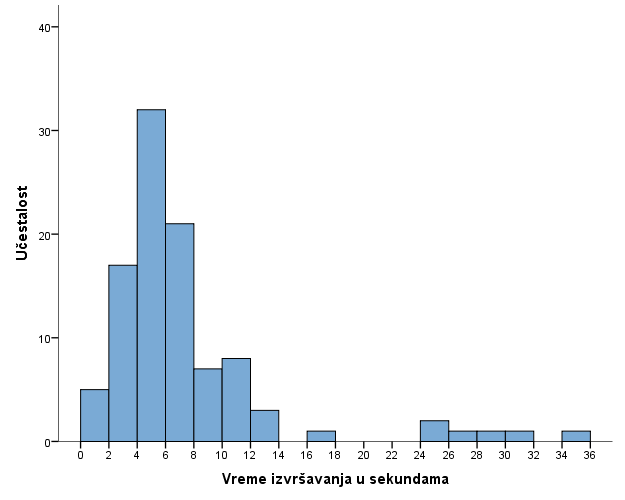
\includegraphics[scale=0.4]{vreme1.png}
	\end{center}
	\caption{{\small Histogram učestalosti vremena izvršavanja za 100 puštanja programa za G3}}
	\label{fig:slika6}
\end{figure}

	\begin{figure}[H]
	\begin{center}
		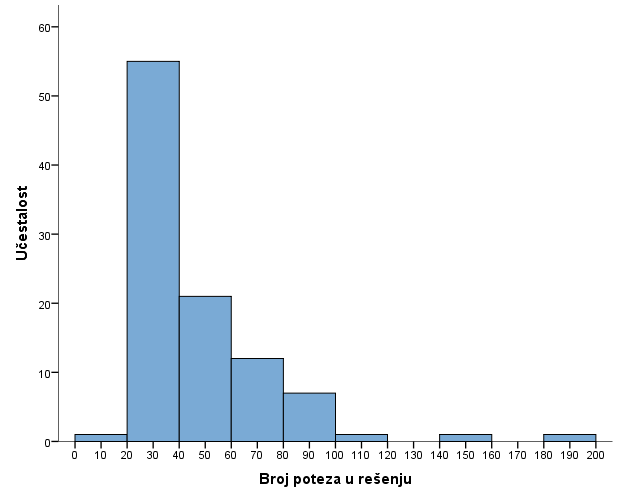
\includegraphics[scale=0.4]{brojpoteza1.png}
	\end{center}
	\caption{{\small Histogram učestalosti broja poteza za 100 puštanja programa za G3}}
	\label{fig:slika7}
\end{figure}

\vspace*{2\baselineskip}

	\section{Zaključak}
	\label{sec:zakljucak}
	
	U ovom radu prikazan je genetski algoritam za rešavanje problema planiranja pokreta u povezanom, neusmerenom grafu. Kao što je prikazano u radu, algoritam se pokazao kao relativno uspešan u rešavanju ovog problema, i u slučaju primera sa puno čvorova, pruža značajno poboljšanje u odnosu na algoritam grube sile. Sa histograma se može zaključiti da u većini slučajeva, algoritam donosi prilično dobre rezultate. S obzirom na kompleksnost problema i činjenicu da nije postojala prethodna literatura na koju smo mogli da se oslonimo pri rešavanju problema, ovaj algoritam predstavlja preliminarno rešenje, koje se sigurno može unaprediti, ali se u ovom slučaju pokazao dovoljno dobrim rešenjem.
	
	\newpage
	
	\addcontentsline{toc}{section}{Literatura}
	\bibliography{seminarski} 
	\bibliographystyle{plain}
	
\end{document}
